\documentclass[12pt]{exam}
\usepackage[phy]{template-for-exam}
\usepackage{tikz,ifthen,multicol,siunitx}
\footer{}{}{}
\header{}{}{}
\shadedsolutions
\printanswers
\usetikzlibrary{shadings,decorations.pathmorphing,arrows.meta,patterns}



\begin{document}

\vspace*{\stretch{1}}

\Large


\paragraph{Task 1}

Find the reading on the spring scale of this setup.  You'll need to make sure to measure the mass of the meter stick.  The meter stick is not rotating, so think about what that means about torque.


\begin{center}
  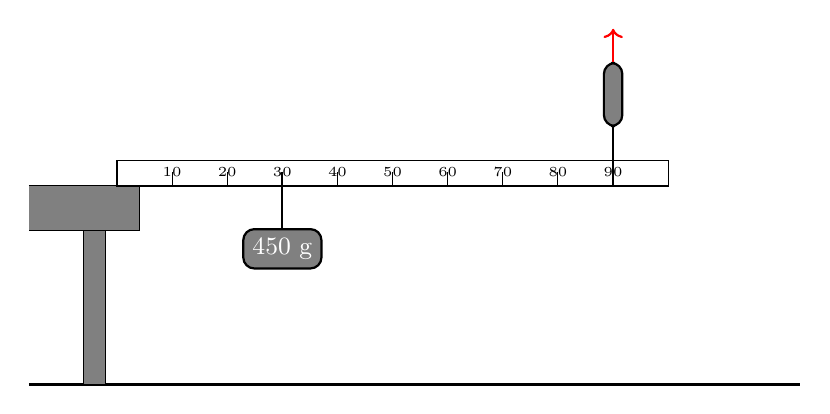
\begin{tikzpicture}[scale=1.4]
    \def\meter{5}
    \draw[thick] (0,0) -- (7,0);
    \draw (0,1.8)
      -- ++ (1,0)
      -- ++ (0,-.4)
      -- ++ (-1,0);
    \fill[gray] (0,1.8) rectangle ++(1,-.4);
    \draw[fill=gray] (0.5,0) rectangle (0.7,1.4);
    \draw (0.8,1.8) coordinate (0) 
      rectangle ++(\meter,0.23);
    \foreach \i in {10,20,30,40,50,60,70,80,90} {
      \draw (0) ++(\i*\meter/100,0) -- ++(0,0.13) 
        node[font=\tiny] (\i) {\i};
    }
  
    \draw[thick] (30.center) -- ++(0,-0.7)
      node[fill=gray, rounded corners, draw=black, text=white, font=\small] {450 g};
  
    \draw[thick] (90.center) -- ++(0,0.7)
      node[fill=gray, rounded corners, draw=black, text=white, minimum height=0.8cm] (scale) {};
    
    \draw[red,thick, ->] 
      (scale.north) -- ++(0,0.3);
  
  \end{tikzpicture}
\end{center}

\vs \hrule \vs

\paragraph{Task 2}

Find the reading for \emph{each} spring scale in this setup. 


\begin{center}
  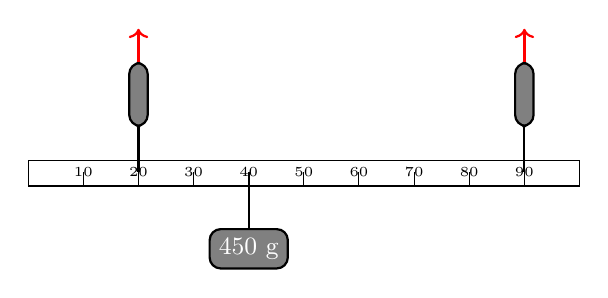
\begin{tikzpicture}[scale=1.4]
    \def\meter{5}
    \draw (0,0) coordinate (0) 
      rectangle ++(\meter,0.23);
    \foreach \i in {10,20,30,40,50,60,70,80,90} {
      \draw (0) ++(\i*\meter/100,0) -- ++(0,0.13) 
        node[font=\tiny] (\i) {\i};
    }
  
    \draw[thick] (40.center) -- ++(0,-0.7)
      node[fill=gray, rounded corners, draw=black, text=white, font=\small] {450 g};
  
    \draw[thick] (20.center) -- ++(0,0.7)
      node[fill=gray, rounded corners, draw=black, text=white, minimum height=0.8cm] (scale) {};
    
    \draw[red,thick, ->] 
      (scale.north) -- ++(0,0.3);
  
    \draw[thick] (90.center) -- ++(0,0.7)
      node[fill=gray, rounded corners, draw=black, text=white, minimum height=0.8cm] (scale) {};
    
    \draw[red,thick, ->] 
      (scale.north) -- ++(0,0.3);
  
  \end{tikzpicture}
\end{center}

\vspace*{\stretch{1}}


\end{document}